\section{Klassische Enterprise-Architektur}


%%%%%%%%%%%%%%%%%%%%%%%%%% Service-oriented Architecture %%%%%%%%%%%%%%%%%%%%%%%%%%
\begin{frame}{Service-oriented Architecture}
  \begin{itemize}
    \item Service:  Dienst, das eine Funktionalität kapselt. Dieser kann aus mehrere Dienste bestehen
    \item Service Provider: Bietet einen spezifischen Dienst an
    \item Service Bus: Dienst, das die Komunikation und Integration zwischen Service Consumer und Service Provider gewährleistet
    \item Service Consumer: Nutzt einen bereitgestelten Dienst, dieses kann einen End-User oder ein anderer Dienst sein
    \item Service Registry: Dient als zentrales Repository, die Informationen über die verfügbare Services speichert (Interface-Vertag + Endpoint)
  \end{itemize}
\end{frame}
\begin{frame}{Service-oriented Architecture: Struktur}

    \begin{figure}[!h]
        \centering
        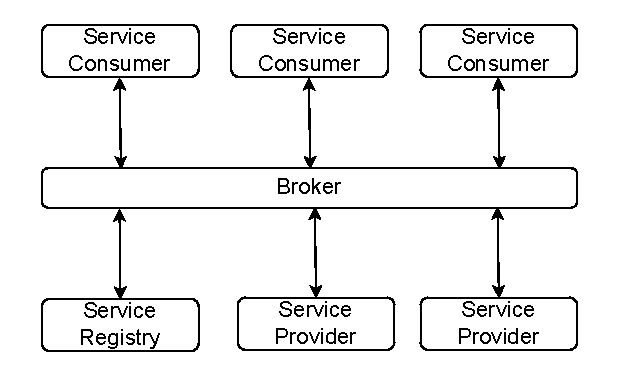
\includegraphics[scale=0.55]{imglib/soa/soa.pdf}
        \caption{Aufbau der Service-oriented Architecture}
        \label{fig:soa}
    \end{figure}
\end{frame}

\begin{frame}{Service-oriented Architecture: Beispiel E-Commerce I}
    \begin{itemize}
        \item \texttt{OrderService}: Ein Dienst, der die Erstellung von Bestellungen übernimmt und dabei den Versand- sowie den Bezahlvorgang automatisch einleitet.in Dienst, das die Erstellung von Bestellung übernimmt. Versandvorgang und Bezahlvorgang werden initiert.
        \item \texttt{PaymentService}: Dienst verantwortlich für die Abwicklung von Zahlungen
        \item \texttt{ShipmentService}: Dienst zuständig für den Versandprozesses
    \end{itemize}
\end{frame}

\begin{frame}{Service-oriented Architecture: Beispiel E-Commerce II}
    \begin{figure}[!h]
        \centering
        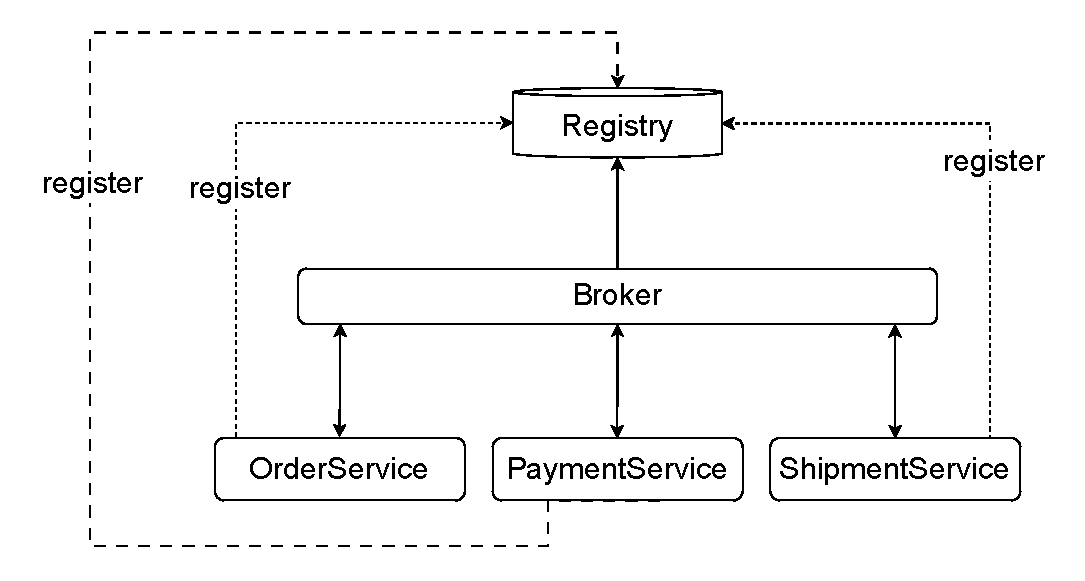
\includegraphics[scale=0.5]{imglib/soa/soa-example.pdf}
        \caption{E-Commerce-Beispiel mit Service-oriented Architecture}
        \label{fig:soaecommerce}
    \end{figure}
\end{frame}

\begin{frame}{Service-oriented Architecture: Agilität}
    \begin{itemize}
        \item Services können unabhängig voneinander parallel entwickelt werden
        \item Interfaces ermöglichen gute Kollaboration im Team
        \item Kundenanforderungen können kurzfristig umgesetzt werden
        \item Zeit- und Kosteneinsparungen durch die Wiederverwendung von Services
        \item Nachteil: Langfristig könnten sich Abhängigkeiten zwischen den Services entwickeln
      \end{itemize}
\end{frame}
